\subsubsection{UC14.2.1 Vis. log della funzione in lista}
\begin{figure}[h]
	\centering
	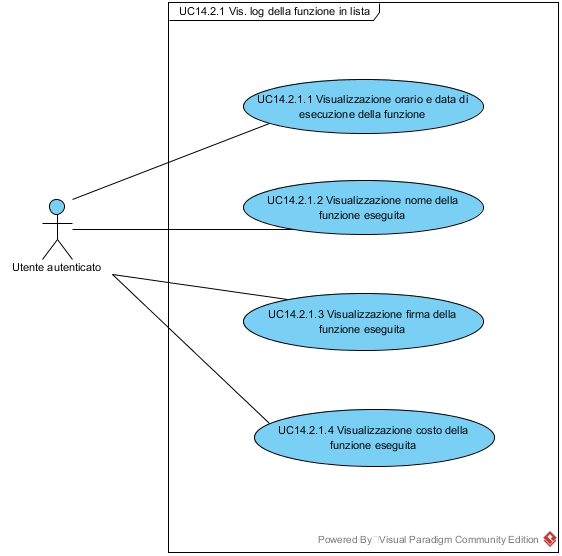
\includegraphics[width=0.7\linewidth]{res/img/UC14.2.1.jpg}
	\caption{Diagramma UC14.2.1 - Visualizzazione della singola funzione in "log"}
\end{figure}
\begin{itemize}
	\item \textbf{Attori primari:} Utente autenticato;
	\item \textbf{Descrizione:} l'utente visualizzerà sul \textit{CLI\glo} i dettagli di una singola funzione;
	\item \textbf{Pre-condizioni:} l'utente ha eseguito il comando "log" e ha visualizzato il log delle funzioni;
	\item \textbf{Post-condizioni:} dettagli di una singola funzione;
	\item \textbf{Scenario principale:} Il sistema mostrerà sulla \textit{CLI\glo} le informazioni relative a una singola funzione.
\end{itemize}
